% \section{TAREAS}
% \begin{itemize}
%     % \item  \textbf{Hacer PPT para el personal del SENA}
%     \item  \textbf{Hacer resumen del trabajo para articulo cientifico}, formato genérico por el momento
%     % \item  \textbf{Hacer 
%     % formulario del trabajo (6 preguntas)}. Hablar  del modelado, del tabajo realizado y la precision del modelo. Posibilidad y trabajos futuros.
%     % \item Corregir preguntas formulario
%     % \item Cuadrar reunion (1 semana de anticipación)

% \end{itemize}

En este capítulo se presenta la evaluación del proyecto en cuanto al cumplimiento de los objetivos del proyecto, así como también con respecto a los análisis planteados en la etapa de preparación de datos y los resultados obtenidos. Para ello es importante citar nuevamente los objetivos específicos planteados al inicio del Capítulo \ref{Objs}:

%\subsection{Objetivos Específicos 10 - 19}
\section{Objetivos específicos (OE)}\label{objesp}
\subsection{OE\#1: Identificar entradas, salidas, variables y parámetros asociados al sistema de producción ganadero objetivo.}

Teniendo en cuenta el proceso descriptivo realizado en los capítulos anteriores, se puede establecer que la información correspondiente al OE\#1 se encuentra resumido de la siguiente manera:

\subsubsection{Entradas}
Son las reses que participan en la producción de leche cruda. Así como también los insumos  que permiten el mantenimiento del CA-SENA-POP.

\subsubsection{Variables}
Las variables en cuestión son, por una parte, la cantidad de leche producida por una vaca durante un periodo de lactancia, por otra parte, la cantidad de peso de la reses productoras o no productoras; y por último, la cantidad de estiércol producido por el hato que será tratado para producir abono para el CA-SENA-POP.

\subsubsection{Salidas}

Las salidas del sistema productivo del CA-SENA-POP son, la producción neta de leche cruda, la producción de carne de las reses vendidas y la producción de estiércol y materia fecal que puede ser usado como abono en los distintos potreros internos en la finca del SENA en la ciudad de Popayán. La leche cruda es producida para posteriormente ser vendida para generar ganancias monetarias que serán reinvertidas en el CA-SENA-POP. La carne representa el peso final de la res parida, desteta, cebada o en proceso de venta. 

\subsubsection{Parámetros}

El sistema productivo del CA-SENA-POP depende del consumo nutricional del hato. Este consumo varía proporcionalmente al peso del animal y a su rendimiento productivo teniendo un rango de valores proporcionales que oscilan de la siguiente manera:
\begin{itemize}
    \item Forrajes y alimentos secos: Consumo que varía entre un 10 a 20 \% del peso del animal.
    \item Concentrado y suplementos: Consumo que varía entre un 1 a 5 \% del peso del animal.
    \item Agua: Consumo ``Ad libitum'', que varía entre un 5 a 12 \% del peso del animal
    \item Medicamentos: Varían según el estado de salud del animal. Se asume un estado de salud óptimo durante este trabajo de investigación.
\end{itemize}

\subsection{OE\#2: Identificar modelos dinámicos que permitan pronosticar la producción de un sistema ganadero objetivo.}

Tal y como se menciona en la Sección \ref{dinamod}, soportado por \cite{shanks}, \cite{silvestre} y \cite{iran}, una forma de encontrar una representación de un sistema por EDOs, es mediante un balance de energía que involucre a las variables en cuestión. Por tal motivo, se puede considerar factible que el modelo de 2 dimensiones descrito en la Sección \ref{edosec} satisface el pronóstico evolutivo de las 3 variables de producción del sistema ganadero en cuestión.


\subsection{OE\#3: Implementar métodos de solución de los modelos dinámicos de producción ganadera seleccionados.}

% Tal y como se concluye en la Sección \ref{simulwp}, una vez que se considera que un modelo EDO puede representar el comportamiento de las variables del sistema, este modelo EDO puede ser resuelto mediante algoritmos numéricos avanzados tales como que pueden ser utilizados mediante librerías como ``Scipy'', en scripts de Python. Para este caso, el sistema modelado en cuestión representa un problema de valor inicial, por lo que puede ser resuelto mediante un método de solución como ``odeint'' o ``scipy.integrate''. El proceso en el que este algoritmo es usado para dar solución al modelo EDO a cada una de las producciones de las reses que pertenecen al sistema se encuentra descrito en la Sección \ref{optimizodeint} o en mayor detalle en los scripts de python implementados en Jupyter-Anaconda \cite{msclfggprogrepo}.

Según se concluye en la Sección \ref{simulwp}, una vez que se determina que un modelo de ecuaciones diferenciales ordinarias (EDO) puede representar el comportamiento de las variables del sistema, es posible resolver dicho modelo utilizando algoritmos numéricos avanzados, como los proporcionados por la biblioteca ``Scipy'' en scripts de Python. En este caso particular, el sistema modelado representa un problema de valor inicial, por lo tanto, se puede resolver mediante métodos de solución como ``odeint'' o ``scipy.integrate''. El proceso en el que se emplea este algoritmo para obtener la solución del modelo de EDO para cada una de las producciones de las reses pertenecientes al sistema está descrito en la Sección \ref{simulwp}, o en mayor detalle, en los scripts de Python implementados en Jupyter-Anaconda. \cite{msclfggprogrepo}.


\subsection{OE\#4: Evaluar la estimación de los modelos seleccionados comparando la solución con datos empíricos recogidos.} 

En cuanto a este objetivo, el modelo WP, planteado por el sistema de 2D de EDOs descrito en el capítulo anterior tiene un desempeño deseado puesto que tal y como se describe en la Sección \ref{visualres}, los valores de los criterios BIC Y AIC son menores a medida que el modelo logra un ajuste más apropiado para cada una de las reses de cada parto. Adicionalmente, criterios como el $\chi^{2}$ reducido tienden a ser cada vez más próximo a 1 lo que complementa la afirmación anterior. Por último pero no menos importante, aún cuando esta última afirmación es netamente subjetiva, se puede observar que  cuando el modelo presenta características estadísticas como las previamente descritas en este objetivo, el ajuste visual tiende a ser similar al comportamiento de los datos empíricos recogidos.



% \section{Objetivo General}
% Estructurar y evaluar un modelo dinámico que simule el comportamiento de sistemas de producción ganadera en el Centro Agropecuario del Servicio Nacional de Aprendizaje, ubicado en el municipio de Popayán, en departamento del Cauca (CA-SENA-POP).

\section{Metodología CRISP-DM}

En lo que respecta a la metodología de estudio, las actividades llevadas a cabo en las etapas de la metodología CRISP-DM descritas en los capítulos anteriores pueden ser justificantes suficientes para corroborar si se ha hecho un debido manejo y procesamiento de datos, en especial, porque cada una de las acciones realizadas al conjunto de datos base ha sido detallada y justificada en cada capítulo en pro de satisfacer los objetivos de este trabajo de grado.\\

De manera general, se puede mencionar que:
\begin{enumerate}
    \item En cuanto al primer objetivo específico (OE\#1), las etapas 1, 2 y 3 de la metodología CRISP-DM permiten identificar el contexto del CA-SENA-POP, así como también los recursos que participan en el proceso productivo del hato.
    \item Para satisfacer el OE\#2, basta con realizar un proceso repetitivo entre las etapas CRISP \#1, \#2, \#3 y \#4; en pro de determinar los parámetros y variables que deben ser tenidos en cuenta al momento de realizar el ajuste de los datos a modelos EDO.
    \item Respecto al OE \#3, éste puede ser satisfecho una vez cumplidas las primeras 3 etapas de la metodología CRISP.
    \item Por último pero no menos importante, el OE \#4 podrá ser satisfecho en el transcurso de esta etapa de evaluación.
\end{enumerate}
 
 


\section{Cumplimiento del OE\#4 en la etapa de Modelación: Ajuste de curvas por métodos no lineales}

\begin{table}[H]
\centering
\caption{Comparación de error cuadrático medio (MSE) para cada método de ajuste no lineal.}
\label{msecompare}
\resizebox{\textwidth}{!}{%
\begin{tabular}{|ccccccc|}
\hline
\multicolumn{7}{|c|}{MSE} \\ \hline
\multicolumn{1}{|c|}{\multirow{2}{*}{\begin{tabular}[c]{@{}c@{}}MÉTODO DE\\ AJUSTE\end{tabular}}} &
  \multicolumn{6}{c|}{PARTO ($P\#_{i}$)} \\ \cline{2-7} 
\multicolumn{1}{|c|}{} &
  \multicolumn{1}{c|}{$P\#_{1}$} &
  \multicolumn{1}{c|}{$P\#_{2}$} &
  \multicolumn{1}{c|}{$P\#_{3}$} &
  \multicolumn{1}{c|}{$P\#_{4}$} &
  \multicolumn{1}{c|}{$P\#_{5}$} &
  $P\#_{6}$ \\ \hline
\multicolumn{1}{|c|}{MA: FU-LM} &
  \multicolumn{1}{c|}{6.8240} &
  \multicolumn{1}{c|}{17.8285} &
  \multicolumn{1}{c|}{21.4705} &
  \multicolumn{1}{c|}{12.4351} &
  \multicolumn{1}{c|}{11.3886} &
  4.8692 \\ \hline
\multicolumn{1}{|c|}{MA: FM} &
  \multicolumn{1}{c|}{4.4826} &
  \multicolumn{1}{c|}{8.444} &
  \multicolumn{1}{c|}{12.7492} &
  \multicolumn{1}{c|}{8.7615} &
  \multicolumn{1}{c|}{9.4352} &
  4.7066 \\ \hline
\multicolumn{1}{|c|}{MA: EF} &
  \multicolumn{1}{c|}{4.4855} &
  \multicolumn{1}{c|}{8.4482} &
  \multicolumn{1}{c|}{12.7476} &
  \multicolumn{1}{c|}{8.7735} &
  \multicolumn{1}{c|}{9.4402} &
  4.6487 \\ \hline
\end{tabular}%
}
\end{table}
\pagebreak

Para realizar una evaluación crítica respecto a los ajustes no lineales de las curvas de lactancia para determinar si estos son representativos y significativos; es necesarios tener en consideración los criterios de MSE, RMSE; para cada uno de los métodos de ajustes no lineales realizados. (Levenberg-Marquardt ó LM, Fit Multiple ó FM, Efectos Mixtos ó EM). \\


\begin{table}[h]
\centering
\caption{Comparación de la raíz del error cuadrático medio (RMSE) para cada método de ajuste no lineal.}
\label{rmsecompare}
\resizebox{\textwidth}{!}{%
\begin{tabular}{|ccccccc|}
\hline
\multicolumn{7}{|c|}{RMSE} \\ \hline
\multicolumn{1}{|c|}{\multirow{2}{*}{\begin{tabular}[c]{@{}c@{}}MÉTODO DE\\ AJUSTE\end{tabular}}} &
  \multicolumn{6}{c|}{PARTO ($P\#_{i}$)} \\ \cline{2-7} 
\multicolumn{1}{|c|}{} &
  \multicolumn{1}{c|}{$P\#_{1}$} &
  \multicolumn{1}{c|}{$P\#_{2}$} &
  \multicolumn{1}{c|}{$P\#_{3}$} &
  \multicolumn{1}{c|}{$P\#_{4}$} &
  \multicolumn{1}{c|}{$P\#_{5}$} &
  $P\#_{6}$ \\ \hline
\multicolumn{1}{|c|}{MA: FU-LM} &
  \multicolumn{1}{c|}{2.6123} &
  \multicolumn{1}{c|}{4.2224} &
  \multicolumn{1}{c|}{4.6336} &
  \multicolumn{1}{c|}{3.5263} &
  \multicolumn{1}{c|}{3.3747} &
  2.2066 \\ \hline
\multicolumn{1}{|c|}{MA: FM} &
  \multicolumn{1}{c|}{2.1172} &
  \multicolumn{1}{c|}{2.9059} &
  \multicolumn{1}{c|}{3.5706} &
  \multicolumn{1}{c|}{2.96} &
  \multicolumn{1}{c|}{3.0717} &
  2.1695 \\ \hline
\multicolumn{1}{|c|}{MA: EF} &
  \multicolumn{1}{c|}{2.1179} &
  \multicolumn{1}{c|}{2.9066} &
  \multicolumn{1}{c|}{3.5704} &
  \multicolumn{1}{c|}{2.962} &
  \multicolumn{1}{c|}{3.0725} &
  2.1561 \\ \hline
\end{tabular}%
}
\end{table}

En primera instancia, los ajustes no lineales realizados al inicio del Capítulo \ref{crisp4} evidencian características estadísticas con valores relativamente bajos de MSE y RMSE (ver Tabla \ref{msecompare} y Tabla \ref{rmsecompare}), así como también una reducción progresiva de los criterios AIC y BIC a medida que se comparan los métodos de ajuste de curvas por los algoritmos de efectos mixtos fijos y aleatorios no lineales (ver Tabla \ref{aicbiccompare} ) .\\

\begin{table}[H]
\centering
\caption{Comparación del Criterio de Información de Akaike (AIC) y el Criterio de Información Bayesiano (BIC) para los métodos de ajuste no lineales por efectos mixtos fijos y aleatorios}
\label{aicbiccompare}
\resizebox{\textwidth}{!}{%
\begin{tabular}{|ccccccc|}
\hline
\multicolumn{1}{|c|}{\multirow{2}{*}{\begin{tabular}[c]{@{}c@{}}MÉTODO DE\\ AJUSTE (MA)\end{tabular}}} &
  \multicolumn{6}{c|}{PARTO ($P\#_{i}$)} \\ \cline{2-7} 
\multicolumn{1}{|c|}{} &
  \multicolumn{1}{c|}{$P\#_{1}$} &
  \multicolumn{1}{c|}{$P\#_{2}$} &
  \multicolumn{1}{c|}{$P\#_{3}$} &
  \multicolumn{1}{c|}{$P\#_{4}$} &
  \multicolumn{1}{c|}{$P\#_{5}$} &
  $P\#_{6}$ \\ \hline
\multicolumn{7}{|c|}{AIC} \\ \hline
\multicolumn{1}{|c|}{MA: EM FIJOS} &
  \multicolumn{1}{c|}{3922.319} &
  \multicolumn{1}{c|}{10130.376} &
  \multicolumn{1}{c|}{11747.833} &
  \multicolumn{1}{c|}{9700.2539} &
  \multicolumn{1}{c|}{3077.2224} &
  1433.494 \\ \hline
\multicolumn{1}{|c|}{MA: EM ALEATORIOS} &
  \multicolumn{1}{c|}{3921.065} &
  \multicolumn{1}{c|}{10118.0196} &
  \multicolumn{1}{c|}{11734.873} &
  \multicolumn{1}{c|}{9700.95} &
  \multicolumn{1}{c|}{3077.2224} &
  1435.2825 \\ \hline
\multicolumn{7}{|c|}{BIC} \\ \hline
\multicolumn{1}{|c|}{MA: EM FIJOS} &
  \multicolumn{1}{c|}{3916.9107} &
  \multicolumn{1}{c|}{10129.9979} &
  \multicolumn{1}{c|}{11747.4544} &
  \multicolumn{1}{c|}{9699.8753} &
  \multicolumn{1}{c|}{3068.0744} &
  1425.6529 \\ \hline
\multicolumn{1}{|c|}{MA: EF ALEATORIOS} &
  \multicolumn{1}{c|}{3914.7556} &
  \multicolumn{1}{c|}{10117.5869} &
  \multicolumn{1}{c|}{11734.4402} &
  \multicolumn{1}{c|}{9700.3623} &
  \multicolumn{1}{c|}{3068.0744} &
  1423.1048 \\ \hline
\end{tabular}%
}
\end{table}

Por lo tanto, es plausible afirmar que los ajustes realizados presentan una buena bondad de ajuste. (Para mayor información respecto a los características estadísticas de cada ajuste, consultar en \cite{msclfggprogrepo}, los scripts de Matlab ``AnaMixEffGenBeta2.m'' y ``lm\_exampGEN2023.m''.\\
% y comparar las estructuras STATSMEFIN, STATSNLME2 y STATSNLME2RF). \\


\subsection{Producción neta real Vs Producción teórica por ajustes no lineales}

Una forma de evaluar la adecuación de los ajustes no lineales de los parámetros del modelo de Wood es mediante la verificación del área bajo la curva generada por estos parámetros. Esta curva representa la producción neta de lactancia, obtenida a partir de los parámetros ajustados al modelo matemático de Wood. Para ello, se puede crear una tabla que contenga los valores de las producciones netas reales de grupo de parto (Producción Real ó PR) y se compare con las producciones netas estimadas (Producción estimada PT) por cada método de ajuste (ó ``Fit''). De esta manera, se puede determinar si los ajustes son capaces de representar los datos de cada vaca y, en última instancia, la producción total del hato. Esta comparación puede apreciarse en la Tabla \ref{prodparamscomparepng}, los valores de producción están en toneladas [t] y el total de ganancia por venta de leche ``$\$\$\$_{Total}$'' está en millones de pesos colombianos [COP].\\

En esta misma Figura se puede observar como el método no lineal que presenta mejor ajuste es el LMA, el cual, aunque no presenta los porcentaje de error más pequeños para todos los grupos de partos, si presenta un valor total más aproximado con respecto a la producción total  real de leche, basada en registros.

% \pagebreak
\subsection{Modelo EDO: Ajuste por mínimos cuadrados}

Tal y como se menciona en la Sección \ref{optimizodeint}, una vez se ha hecho el llamado al solucionador de EDO ``odeint'' restringiendo los valores de cada parámetro $k_{i}$, se pueden obtener los parámetros que permiten el ajuste del modelo EDO a los datos de peso W y de materia producida P=L+E. \\

Según se explica en el apartado de resultados de esa misma Sección, se puede ver como el modelo presenta una bondad de ajuste apropiada que, aunque no aplica para todas las reses de todos los partos, posee buenos criterios estadísticos como los criterios AIC y BIC bastante reducidos entre mejor es el ajuste, así como también un valor de $\chi^{2}$ reducido cercano a 1 (ver Figura \ref{ajustemodSolstatspng}). Por último pero no menos importante, se observa como para algunas reses en cada parto, los parámetros $k_{i}$ poseen errores relativos inferiores al 20\% lo que podría considerarse como un buen ajuste generalizado. \\

Es importante mencionar que el modelo EDO-WP si bien puede presentar un buen ajuste para los datos asociados a algunas reses, no es un modelo perfecto por lo que no es sorpresa evidenciar que el modelo no presenta un buen ajuste para todas las reses. No obstante, esta observación también esta condicionada al hecho que no se cuentan con los datos apropiados de peso y producción de estiércol, lo que dificulta brindar un ajuste preciso para datos faltantes o especulativos.\\

Con base en lo anterior se puede establecer que el OE \#3 ha sido cumplido, en tanto que la solución numérica del modelo, permite lograr un ajuste bondadoso a los datos existentes. De igual manera se establece que el OE\#4 ha sido cumplido en tanto que el modelo EDO-WP ha sido evaluado con respecto a los datos empíricos recogidos, al mostrar buenas características estadísticas que permiten afirmar que presenta un buen ajuste respecto a los datos usados.

\pagebreak

%%%%% Solo las producciones por cada grupo de parto
%%%%%
% \begin{sidewaystable}%[H]
\begin{table}
\centering
\caption{Comparación de producción real y teórica para cada método de modelación utilizada.} \label{prodparamscomparepng}
\resizebox{\textwidth}{!}{\begin{tabular}{|cc|c|c|c|c|c|c|c|c|c|c|c|}
 % $PR_{P\#_{i}}$ - NETA [Kg]
 % PRvs.\PT - NETA [Kg]
 % \cellcolor[HTML]{FFD9AC}
    \hline
     \cellcolor[HTML]{EBEBEB} &\cellcolor[HTML]{EBEBEB} & \cellcolor[HTML]{FFD9AC}$Prod_{Real}$ & \cellcolor[HTML]{BBFFBB} LMA &\cellcolor[HTML]{BBFFBB} $\%_{Error}$ & \cellcolor[HTML]{EBEBEB} $S_{Vaca}$ &\cellcolor[HTML]{EBEBEB} $\%_{Error}$ & \cellcolor[HTML]{EBEBEB} NLMEA-F & \cellcolor[HTML]{EBEBEB} $\%_{Error}$ & \cellcolor[HTML]{EBEBEB} NLMEA-R & \cellcolor[HTML]{EBEBEB} $\%_{Error}$ & \cellcolor[HTML]{FFD2B7} EDO-WP & \cellcolor[HTML]{FFD2B7}$\%_{Error}$\\  
     % ``FIT''-EDO & \cellcolor[HTML]{EBEBEB}$\%_{Error}$\\ 
     \cellcolor[HTML]{EBEBEB}PARTO $P\#_{i}$ & \cellcolor[HTML]{EBEBEB}N & \cellcolor[HTML]{FFD9AC} $PR_{P\#_{i}}$ & \cellcolor[HTML]{BBFFBB} PT & \cellcolor[HTML]{BBFFBB} & \cellcolor[HTML]{EBEBEB} PT & \cellcolor[HTML]{EBEBEB} & \cellcolor[HTML]{EBEBEB} PT & \cellcolor[HTML]{EBEBEB} & \cellcolor[HTML]{EBEBEB} PT  & \cellcolor[HTML]{EBEBEB} & \cellcolor[HTML]{FFD2B7} PT  & 
     %\cellcolor[HTML]{EBEBEB}  \\
     \cellcolor[HTML]{FFD2B7}  \\
     % & \cellcolor[HTML]{EBEBEB} (PRvs\ PT) & \cellcolor[HTML]{EBEBEB} PT & \cellcolor[HTML]{EBEBEB} (PRvs\ PT) & \cellcolor[HTML]{EBEBEB} PT & \cellcolor[HTML]{EBEBEB} (PRvs\ PT) & \cellcolor[HTML]{EBEBEB} PT  & \cellcolor[HTML]{EBEBEB} (PRvs\ PT) & \cellcolor[HTML]{EBEBEB} PT  & \cellcolor[HTML]{EBEBEB} (PRvs\ PT)  \\
     \hline
     
     \cellcolor[HTML]{343434} \color[HTML]{FFFFFF}$P\#_{1}$ & \cellcolor[HTML]{656565} \color[HTML]{FFFFFF}299 & \cellcolor[HTML]{FFD9AC}8.873 & \cellcolor[HTML]{BBFFBB}8.885 & \cellcolor[HTML]{BBFFBB}0.146\%& 8.876 & 0.041\% & 8.877 & 0.045\% & 8.912 & 0.449\% & \cellcolor[HTML]{FFD2B7}8.215 & \cellcolor[HTML]{FFD2B7}7.412\%\\
     
     \hline
     
     \cellcolor[HTML]{3241CB}\color[HTML]{FFFFFF}$P\#_{2}$ & \cellcolor[HTML]{BDFFFC}288 & \cellcolor[HTML]{FFD9AC}24.712 & \cellcolor[HTML]{BBFFBB}24.751 & \cellcolor[HTML]{BBFFBB}0.158\%& 24.800 & 0.357\% & 24.835 & 0.501\% & 24.844 & 0.534\% & \cellcolor[HTML]{FFD2B7}24.28 & \cellcolor[HTML]{FFD2B7}1.745\%\\
     
     \hline
     
     \cellcolor[HTML]{32CB00}$P\#_{3}$ & \cellcolor[HTML]{AAFF85}309 & \cellcolor[HTML]{FFD9AC}33.097 & \cellcolor[HTML]{BBFFBB}33.102 & \cellcolor[HTML]{BBFFBB}0.015\% & 33.114 & 0.052\% & 33.123 & 0.079\% & 33.130 & 0.049\% & \cellcolor[HTML]{FFD2B7}35.129 & \cellcolor[HTML]{FFD2B7}6.142\%\\
     
     \hline
     
     \cellcolor[HTML]{FFFE65}$P\#_{4}$ & \cellcolor[HTML]{FFFFC7}274 & \cellcolor[HTML]{FFD9AC}20.696 & \cellcolor[HTML]{BBFFBB}20.686 & \cellcolor[HTML]{BBFFBB}0.045\% & 20.722 & 0.129\% & 20.725 & 0.144\% & 20.731 & 0.173\% & \cellcolor[HTML]{FFD2B7}20.114 & \cellcolor[HTML]{FFD2B7}2.809\%\\
     
     \hline
     
     \cellcolor[HTML]{D34444}$P\#_{5}$ & \cellcolor[HTML]{FFCCC9}298 & \cellcolor[HTML]{FFD9AC}7.111 & \cellcolor[HTML]{BBFFBB}7.154 & \cellcolor[HTML]{BBFFBB}0.604\% & 7.126 & 0.217\% & 7.136 & 0.354\% & 7.138 & 0.384\% & \cellcolor[HTML]{FFD2B7}7.125 & \cellcolor[HTML]{FFD2B7}0.198\%\\
     
     \hline
     
     \cellcolor[HTML]{6665CD}$P\#_{6}$ & \cellcolor[HTML]{CBCEFB}162 & \cellcolor[HTML]{FFD9AC}6.2707 & \cellcolor[HTML]{BBFFBB}6.2700 & \cellcolor[HTML]{BBFFBB}0.013\% & 6.2705 & 0.004\% & 6.2705 & 0.004\% & 6.269 & 0.017\% & \cellcolor[HTML]{FFD2B7}6.287 & \cellcolor[HTML]{FFD2B7}0.271\%\\
     
     \hline
     \hline
     \hline
     
     %  &  &  & & & & & & & & & & \\

     % \hline
     
     \cellcolor[HTML]{EBEBEB}$P_{TOTAL}$ & \cellcolor[HTML]{EBEBEB}[t] & \cellcolor[HTML]{FFD9AC}100.760 & \cellcolor[HTML]{BBFFBB}100.850 & \cellcolor[HTML]{BBFFBB}0.089\% & 100.911 & 0.150\% & 100.968 & 0.207\% & 101.027 & 0.265\% & \cellcolor[HTML]{FFD2B7}101.153 & \cellcolor[HTML]{FFD2B7}0.391\% \\

     \hline
     
     \cellcolor[HTML]{EBEBEB}$\$\$\$_{TOTAL}$ & \cellcolor[HTML]{EBEBEB}[COP] & \cellcolor[HTML]{FFD9AC}136.026 & \cellcolor[HTML]{BBFFBB}136.147 & \cellcolor[HTML]{BBFFBB} 0.089\%& 136.230 & 0.150\% & 136.307 & 0.207\% & 136.386 & 0.265\% & \cellcolor[HTML]{FFD2B7}136.557 & \cellcolor[HTML]{FFD2B7} 0.391\%\\
     % \cellcolor[HTML]{FFD9AC}$\$\$\$_{TOTAL}$ & \cellcolor[HTML]{FFD9AC} & 6.2707 & 6.2700 &  & 6.2705 &  & 6.2705 &  & 6.269 &  & 6.287 & \\
     \hline

     % \hline
     
 \end{tabular}}
 \\
\end{table}
% \end{sidewaystable}
%%%%%
%%%%%

%%%%%% con cada una de las vacas
%%%%%%
% \begin{sidewaystable}%[H]
% % \begin{table}
% \centering
% \caption{Comparación de producción real y teórica para cada método de modelación utilizada.} \label{prodparamscomparepng}
% \resizebox{0.95\textwidth}{!}{\begin{tabular}{|cc|c|c|c|c|c|c|c|c|c|c|c|c|}
%  % $PR_{P\#_{i}}$ - NETA [Kg]
%  % PR vs.\ PT - NETA [Kg]
%     \hline
%      \cellcolor[HTML]{FFD9AC} &  \cellcolor[HTML]{FFD9AC} &\cellcolor[HTML]{FFD9AC} & \cellcolor[HTML]{FFD9AC}Registros & \cellcolor[HTML]{FFD9AC} ``FIT''-LM &\cellcolor[HTML]{FFD9AC} $\%_{Error}$ & \cellcolor[HTML]{FFD9AC} ``FIT''-UNICO &\cellcolor[HTML]{FFD9AC} $\%_{Error}$ & \cellcolor[HTML]{FFD9AC} ``FIT''-EM F & \cellcolor[HTML]{FFD9AC} $\%_{Error}$ & \cellcolor[HTML]{FFD9AC} ``FIT''-EM A & \cellcolor[HTML]{FFD9AC} $\%_{Error}$ & \cellcolor[HTML]{FFD9AC} ``FIT''-EDO & \cellcolor[HTML]{FFD9AC}$\%_{Error}$\\  
%      \cellcolor[HTML]{FFD9AC}PARTO $P\#_{i}$ & \cellcolor[HTML]{FFD9AC}N & \cellcolor[HTML]{FFD9AC}VARS & \cellcolor[HTML]{FFD9AC} $PR_{P\#_{i}}$ & \cellcolor[HTML]{FFD9AC} PT & \cellcolor[HTML]{FFD9AC} (PRvs.\ PT) & \cellcolor[HTML]{FFD9AC} PT & \cellcolor[HTML]{FFD9AC} (PRvs.\ PT) & \cellcolor[HTML]{FFD9AC} PT & \cellcolor[HTML]{FFD9AC} (PRvs.\ PT) & \cellcolor[HTML]{FFD9AC} PT  & \cellcolor[HTML]{FFD9AC} (PRvs.\ PT) & \cellcolor[HTML]{FFD9AC} PT  & \cellcolor[HTML]{FFD9AC} (PRvs.\ PT)  \\
%      \cellcolor[HTML]{FFD9AC} & \cellcolor[HTML]{FFD9AC} & \cellcolor[HTML]{FFD9AC}VACA &\cellcolor[HTML]{FFD9AC} &\cellcolor[HTML]{FFD9AC} &\cellcolor[HTML]{FFD9AC} &\cellcolor[HTML]{FFD9AC} &\cellcolor[HTML]{FFD9AC} &\cellcolor[HTML]{FFD9AC} &\cellcolor[HTML]{FFD9AC} & \cellcolor[HTML]{FFD9AC}&\cellcolor[HTML]{FFD9AC} & \cellcolor[HTML]{FFD9AC}& \cellcolor[HTML]{FFD9AC} \\
     
%      \hline
     
%      \cellcolor[HTML]{343434} & \cellcolor[HTML]{343434} & \cellcolor[HTML]{656565}\color[HTML]{FFFFFF}ACER &  &  &  &  &  &  &  &  &  &  & \\
%      \cellcolor[HTML]{343434} \color[HTML]{FFFFFF}$P\#_{1}$ & \cellcolor[HTML]{343434} \color[HTML]{FFFFFF}299 & \cellcolor[HTML]{656565}\color[HTML]{FFFFFF}SOL & 8.873 & 8.885 &  & 8.876 &  & 8.877 &  & 8.912 &  & 8.215 & \\
%      \cellcolor[HTML]{343434} & \cellcolor[HTML]{343434} & \cellcolor[HTML]{656565}\color[HTML]{FFFFFF}LUN &  &  &  &  &  &  &  &  &  &  & \\
     
%      \hline
     
%      \cellcolor[HTML]{3241CB}& \cellcolor[HTML]{3241CB}& \cellcolor[HTML]{BDFFFC}DIAN &  &  &  &  &  &  &  &  &  &  & \\
%      \cellcolor[HTML]{3241CB}& \cellcolor[HTML]{3241CB}& \cellcolor[HTML]{BDFFFC}GINA &  &  &  &  &  &  &  &  &  &  & \\
%      \cellcolor[HTML]{3241CB}& \cellcolor[HTML]{3241CB}& \cellcolor[HTML]{BDFFFC}JUAN &  &  &  &  &  &  &  &  &  &  & \\
%      \cellcolor[HTML]{3241CB}\color[HTML]{FFFFFF}$P\#_{2}$ & \cellcolor[HTML]{3241CB}\color[HTML]{FFFFFF}288 & \cellcolor[HTML]{BDFFFC}LUCI & 24.712 & 24.751 & & 24.800 &  & 24.835 &  & 24.844 &  & 24.28 & \\
%      \cellcolor[HTML]{3241CB}& \cellcolor[HTML]{3241CB}& \cellcolor[HTML]{BDFFFC}PAC &  &  &  &  &  &  &  &  &  &  & \\
%      \cellcolor[HTML]{3241CB}& \cellcolor[HTML]{3241CB}& \cellcolor[HTML]{BDFFFC}SOL &  &  &  &  &  &  &  &  &  &  & \\
%      \cellcolor[HTML]{3241CB}& \cellcolor[HTML]{3241CB}& \cellcolor[HTML]{BDFFFC}VIV &  &  &  &  &  &  &  &  &  &  & \\
     
%      \hline
     
%     \cellcolor[HTML]{32CB00} & \cellcolor[HTML]{32CB00}& \cellcolor[HTML]{AAFF85}FER &  &  &  &  &  &  &  &  &  &  & \\
%      \cellcolor[HTML]{32CB00}& \cellcolor[HTML]{32CB00}& \cellcolor[HTML]{AAFF85}GPA &  &  &  &  &  &  &  &  &  &  & \\
%      \cellcolor[HTML]{32CB00}& \cellcolor[HTML]{32CB00}& \cellcolor[HTML]{AAFF85}JUAN &  &  &  &  &  &  &  &  &  &  & \\
%      \cellcolor[HTML]{32CB00}$P\#_{3}$ & \cellcolor[HTML]{32CB00}309 & \cellcolor[HTML]{AAFF85}LETI & 33.097 & 33.102 &  & 33.114 &  & 33.123 &  & 33.130 &  & 35.129 & \\
%      \cellcolor[HTML]{32CB00}& \cellcolor[HTML]{32CB00}& \cellcolor[HTML]{AAFF85}MART &  &  &  &  &  &  &  &  &  &  & \\
%      \cellcolor[HTML]{32CB00}& \cellcolor[HTML]{32CB00}& \cellcolor[HTML]{AAFF85}MOR &  &  &  &  &  &  &  &  &  &  & \\
%      \cellcolor[HTML]{32CB00}&\cellcolor[HTML]{32CB00} & \cellcolor[HTML]{AAFF85}SOL &  &  &  &  &  &  &  &  &  &  & \\
     
%      \hline
     
%      \cellcolor[HTML]{FFFE65}& \cellcolor[HTML]{FFFE65}& \cellcolor[HTML]{FFFFC7}CENT &  &  &  &  &  &  &  &  &  &  & \\
%      \cellcolor[HTML]{FFFE65}& \cellcolor[HTML]{FFFE65}& \cellcolor[HTML]{FFFFC7}DIAN &  &  &  &  &  &  &  &  &  &  & \\
%      \cellcolor[HTML]{FFFE65}&\cellcolor[HTML]{FFFE65} & \cellcolor[HTML]{FFFFC7}LETI &  &  &  &  &  &  &  &  &  &  & \\
%      \cellcolor[HTML]{FFFE65}$P\#_{4}$ & \cellcolor[HTML]{FFFE65}274 & \cellcolor[HTML]{FFFFC7}MOR & 20.696 & 20.686 &  & 20.722 &  & 20.725 &  & 20.731 &  & 20.114 & \\
%      \cellcolor[HTML]{FFFE65}& \cellcolor[HTML]{FFFE65}& \cellcolor[HTML]{FFFFC7}MUC &  &  &  &  &  &  &  &  &  &  & \\
%      \cellcolor[HTML]{FFFE65}& \cellcolor[HTML]{FFFE65}& \cellcolor[HTML]{FFFFC7}SOR &  &  &  &  &  &  &  &  &  &  & \\
%      \cellcolor[HTML]{FFFE65}& \cellcolor[HTML]{FFFE65}& \cellcolor[HTML]{FFFFC7}VIV &  &  &  &  &  &  &  &  &  &  & \\
     
%      \hline
     
%      \cellcolor[HTML]{D34444}$P\#_{5}$ & \cellcolor[HTML]{D34444}298 & \cellcolor[HTML]{FFCCC9}GPA & 7.111 & 7.154 &  & 7.126 & & 7.136 &  & 7.138 &  & 7.125 & \\
%      \cellcolor[HTML]{D34444}& \cellcolor[HTML]{D34444}& \cellcolor[HTML]{FFCCC9}ANDRE &  &  &  &  &  &  &  &  &  &  & \\
     
%      \hline
     
%      \cellcolor[HTML]{6665CD}$P\#_{6}$ & \cellcolor[HTML]{6665CD}162 & \cellcolor[HTML]{CBCEFB}GPA & 6.2707 & 6.2700 &  & 6.2705 &  & 6.2705 &  & 6.269 &  & 6.287 & \\
%      \cellcolor[HTML]{6665CD}&\cellcolor[HTML]{6665CD} & \cellcolor[HTML]{CBCEFB}ANDRE &  &  &  &  &  &  &  &  &  &  & \\
     
%      \hline
     
%  \end{tabular}}
% % \end{table}
% \end{sidewaystable}
%%%%%%
%%%%%%

% \begin{figure}[H]
%     \centering
%     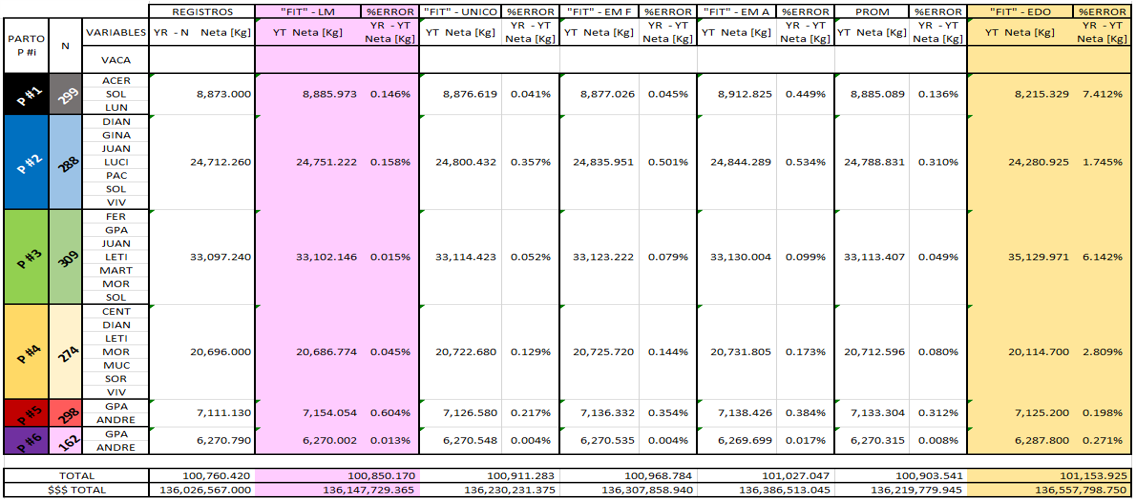
\includegraphics[angle=-90, scale=0.56]{img/prodparamscompare.png}
%     \caption{Comparación de producción real y teórica para cada método de ajuste no lineal. \label{prodparamscomparepng}}
% \end{figure}
\pagebreak

\section{Retroalimentación del proyecto con el cliente final}

El desarrollo de este trabajo pudo ser llevado a cabo tras recibir una respuesta positiva por parte de un cliente (CA-SENA-POP) quien vió en este trabajo de grado, la oportunidad de iniciar un proceso de tecnificación enfocada hacia la industria 4.0 en el sector agropecuario; mediante un proyecto de investigación. Este cliente fue quien proporcionó los espacios y sobretodo los datos que permitieron que los conocimientos del estudiante de maestría, el \authorA, pudieran ser puestos en practica. Como  medida de evaluación del proyecto se considera pertinente tener en consideración la opinión que el cliente pueda tener respecto a cómo se trataron sus datos y qué resultados fueron obtenidos gracias a estos debido al proyecto de investigación llevado a cabo.\\

Por tal motivo, a continuación se describen los espacios de socialización que fueron llevados a cabo con el personal del CA-SENA-POP.



\subsection{Socialización del proyecto con el CA-SENA-POP}
\subsubsection{Socialización Virtual: Miércoles 10 de Mayo de 2023}
Para esta primer socialización se contó con la asistencia de la coordinadora de formación profesional integral Maria del Carmen Agredo, el coordinador del centro agropecuario Daniel Cobo, el profesor y tutor, \director \hspace{0.1cm} y el \authorA, \hspace{0.1cm}quien realiza el proyecto. En esta reunión de poco mas de 20 minutos, se mostró cómo se usaron los datos oficiales proporcionados para que fueran procesados, analizados y clasificados para posteriormente estimar parámetros, realizar ajuste de datos; y finalmente establecer un modelo por EDOs que permitiese predecir el comportamiento de las variables de interés (Ver Figura \ref{tesispptsenapng}). (La presentación usada puede ser encontrada en el repositorio \cite{msclfggrepo}).

Durante esta sesión, la coordinadora Maria del Carmen manifestó una opinión positiva respecto al desarrollo del proyecto, pues según sus palabras, aunque el SENA posee los recursos económicos y humanos para tecnificar su producción ganadera; no cuenta con un proceso sistemático ni con estudios de investigación a nivel de posgrado que soporten la toma de decisiones a futuro. 
En cuanto al manejo y procesamiento de los datos, el SENA se mostró satisfecho al ver que las interpretaciones sobre el conjunto de datos han sido apropiadas y acordes a lo que se maneja en el SENA en tanto que no se realizan suposiciones alejadas de la realidad y fueron soportadas por análisis pertinentes por parte del ingeniero Guevara.\\

Finalmente, la coordinadora Maria del Carmen y el coordinador Daniel Cobo manifestaron en su calidad como representantes del CA-SENA-POP, tener las puertas abiertas para formar una articulación entre la Pontificia Universidad Javeriana Cali y el SENA Popayán, pues manifiestan estar satisfechos con el proyecto de investigación realizado y esperan que futuros proyectos de pregrado o posgrado puedan ser llevados entre las 2 instituciones.
Al finalizar la reunión, la señora Agredo solicitó una segunda reunión de manera presencial en la ciudad de Popayán para que los resultados númericos y visuales puedan ser expuestos al personal del CA-SENA-POP, en especial a la veterinaria Ana Maria Dorado quen no pudo asistir sino hasta el final de la reunión y quien junto con el señor Cobo, dirigen el centro agropecuario y sus intereses como cliente final de este estudio.

% \begin{figure}[H]
%     \centering
%     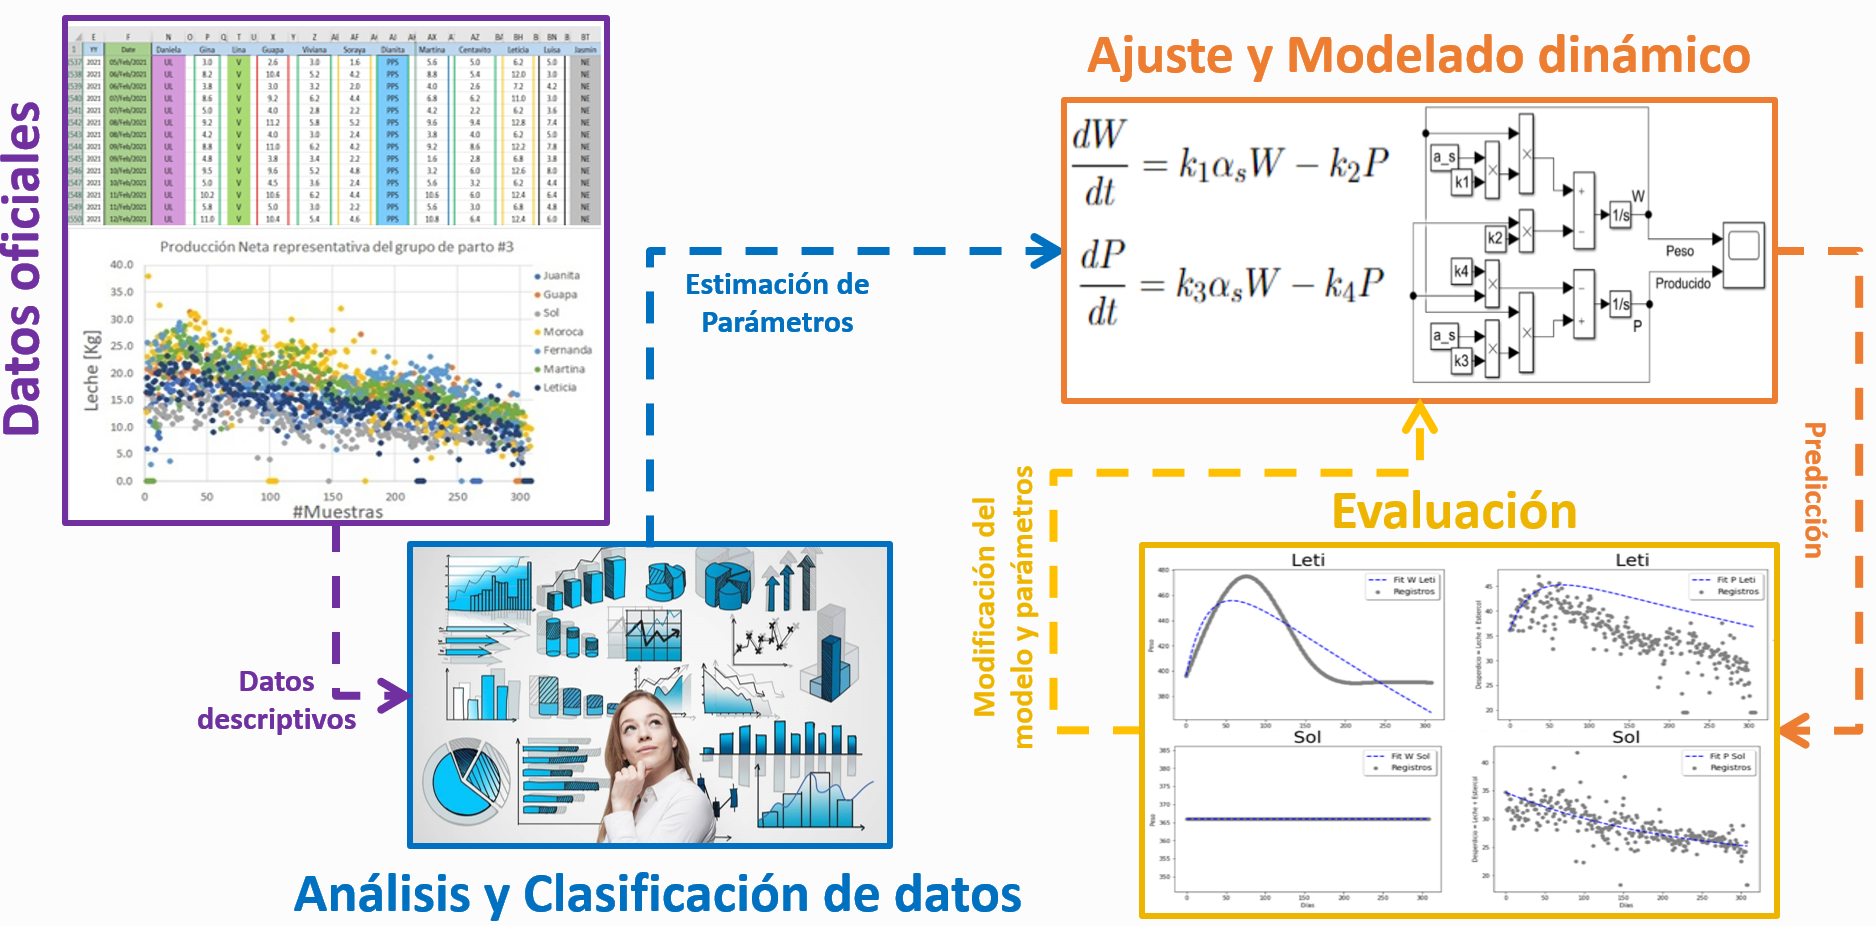
\includegraphics[width=\textwidth]{img/tesispptsena.png}
%     \caption{Planteamiento general de la metodología usada en la ejecución del proyecto}
%     \label{tesispptsenapng}
% \end{figure}

\subsubsection{Socialización presencial: Viernes 19 de Mayo de 2023}


Para esta segunda reunión, nuevamente se muestran los resultados del proyecto de manera que se pudieran evidenciar las virtudes y bondades que ofrece el modelamiento dinámico de sistemas de producción ganadera; y cómo este tipo de modelamiento permitiría pronosticar de manera aproximada el comportamiento productivo del sistema ganadero del SENA y de otros centros agropecuarios del país. Nuevamente, el personal directivo del SENA expresa su satisfacción respecto a los resultados expuestos y mediante una corta encuesta manifiesta tener una aceptación positiva del proyecto dando por terminada la sesión de retroalimentación del proyecto. \\ 

Adicionalmente manifiestan que, aún cuando se cumplen con los objetivos y alcance de este proyecto, quedan expectantes ante futuros proyectos de investigación en el sector agropecuario; pues manifiestan que el SENA cuenta con los recursos biológicos y los espacios interdisciplinares apropiados para que el cuerpo estudiantil de la PUJ pueda poner en práctica sus proyectos de integración profesional en caso que lo requieran y lograr así una articulación educativa entre las 2 instituciones.
